\chapter{Automatic Captioning Pipeline: Model, Data and Evaluation}
\label{chapter:baseline}
%%===========================================================================%%
In this chapter, we will examine in detail all the constituent parts
of training an image captioning system.
%%
First we will look at a baseline captioning model adapted from
\cite{Vinyals_2015_CVPR}. 
%%
Although the original model was proposed for generating captions for still
images, the same architecture can be used for video captioning, by
swapping out the image feature extraction module with video feature extraction
module.
%%
Thus the discussion presented here is kept generic, and specific details of
features used for image or video captioning is discussed in
Chapter~\ref{chapter:VisFeatChapter}.
%%

We will then discuss some popular datasets which are used to train the
captioning models and discuss the salient aspects of each dataset.
%%
We will also discuss the metrics used to evaluate the captions generated by the
models. 

The model presented in this chapter acts as the baseline against which we
compare the improvements presented in the rest of the thesis.

\section{Baseline Architecture} 

Our caption generation model consists of two stages: the visual
feature extraction stage followed by a language model
%%
In the first stage, we use various techniques to extract descriptors of
the visual contents of input image or video.
%%
These descriptors are then represented as one or more vectors of fixed
dimension.
%%
The language model then uses these feature vectors and generates a
suitable caption to describe the image.
%%
This pipeline is illustrated in Figure~\ref{fig_fullModel}. 
%%

In the following subsections we will discuss in detail the different
image features and the language model architectures we have
experimented with.

\begin{figure*}[t]
  \begin{center}
      \hspace{-10mm}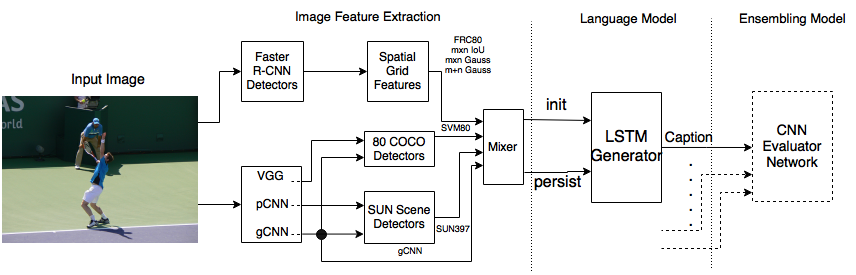
\includegraphics[width=1.2\linewidth]{images/AcMM_fullModel.png}
  \end{center}
  \vspace*{-3mm}
  \caption{Block diagram showing our image captioning pipeline from an
  input image to the generated caption.\red{Update to be more generic}}
  \label{fig_fullModel}
\end{figure*}

\fixme{Upto 3 pages, from ACMMM paper and Project Report}

\subsection{Image Feature extraction}


%%----------------------------------%%
\subsection{Recurrent Language Model}
%%----------------------------------%%
Recurrent Neural networks(RNN) are a good match for the language modeling
problem as they have infinite depth in time in a sense, allowing a RNN based
language model to utilize preceding context when making predictions. This is
because the current state of a RNN, $h_t$ depends on its previous state,
$h_{t-1}$, and thereby on all its previous inputs, $x_t$. This is described in
equations \ref{eq:rnn_h} and \ref{eq:rnn_y}. Here N is the hidden layer
non-linearity and $y_t$ is the network output at time t.

\begin{eqnarray}
    \label{eq:rnn_h} h_t &=& N(W_{xh}x_t+W_{hh}h_{t-1}+b_h)\\
    \label{eq:rnn_y} y_t &=& W_{hy}h_t + b_y
\end{eqnarray} 

A powerful class of recurrent networks called Long Short-Term Memory
(LSTM) models \cite{Hochreiter:1997:LSM:1246443.1246450} are widely used in
image captioning problems today.
Each LSTM unit has a memory cell whose update is controlled by a set of
non-linear gates as shown in figure \ref{fig_lstmcell}. This allows the network
to store important information for a long duration in time, giving them ability
to better handle longer sequences. This model also addresses the problem of
vanishing gradients observed when training vanilla RNN models
\cite{Bengio93Vanishing}\cite{pascanu2012difficulty}.

\begin{figure}[h]
	\begin{center}
		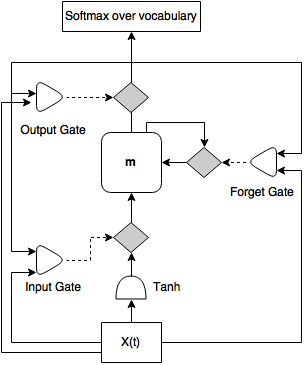
\includegraphics[width=0.5\linewidth]{images/LstmCell.png}
	\end{center}
	\caption{Block diagram of a single LSTM cell. dotted lines indicate
		gate controls and solid lines are data flow. Triangle indicates
		sigmoid non-linearity.}
	\label{fig_lstmcell}
\end{figure}

In an LSTM cell the update to the memory value $m$ is controlled using the
input gate and the forget gate.  The output is controlled using the output
gate. The gate outputs are not binary and are instead implemented using sigmoidal
non-linearity, and thus are differentiable w.r.t the inputs. 
%%
The input and forget gates give the LSTM units the ability to preserve the
content of their memory cells over long periods making it easier to learn
longer patterns.
%%
This process is formalized in the equations below.

\begin{align}
	i(t) &= \sigma(W_{ix}x(t-1) + W_{iy}y(t-1))\\
	o(t) &= \sigma(W_{ox}x(t-1) + W_{oy}y(t-1))\\
	f(t) &= \sigma(W_{fx}x(t-1) + W_{fy}y(t-1))\\
	m(t) &= f(t)\cdot m(t-1) + i(t)\cdot \tanh(W_{mx}x(t)+W_{my}y(t-1))\\
	y_{lstm}(t) &= o(t) \cdot m(t)
\end{align}


\subsection{Training and Regularization}
%%----------------------------------%%
\subsection{Test Mode: Beam Search}
%%----------------------------------%%
\subsection{Implementation Platform Details}
%%----------------------------------%%
%%===========================================================================%%
\section{Datasets}
\fixme{Upto 4 pages, mostly fresh writing, but parts can be taken from previous
papers}
\subsection{MS-COCO}
\subsection{LSMDC}
\subsection{MSR-VTT}
\subsection{Other Datasets}
%%===========================================================================%%
\section{Evaluation Metrics}
The evaluation of a captioning system is not trivial, due to the
\red{multiple} nature of the problem.
%%
An image can be correctly described with wide variety of captions differing not
only in the syntactic structure of the caption, but also in the semantic content
of it.
%%
We can see an example of this in figure~\ref{fig_capdiversity}, where a sample
image from MS-COCO training set is shown with the corresponding ground truth
captions.
%%
Here we see that each caption focusses on different aspects of the image, from
the \emph{big rock} to \emph{crystal blue water}.
%%
But all the captions are equally valid.
%%

One possible method of evaluation is to compare the machine generated
caption with the target reference captions.
%%
But, we need to note that the reference captions only represent few samples from
the space of all valid captions for input image.
%%
Thus the evaluation metrics we use to measure the correctness of a machine
generated caption should be able to take these issues into account.

\begin{figure*}[t]
    \begin{minipage}[c]{0.5\linewidth}
        %\begin{center}
            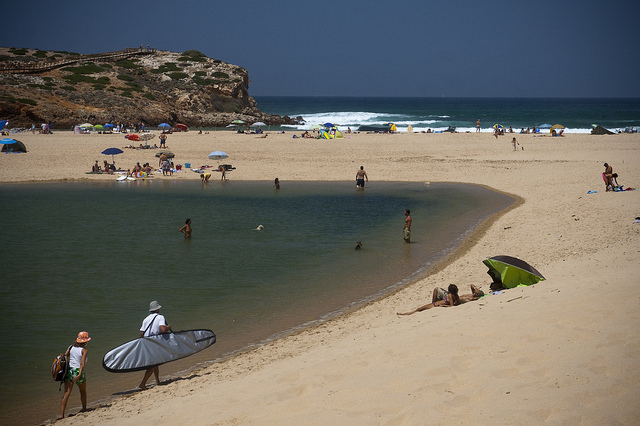
\includegraphics[width=\textwidth]{images/COCO_train2014_000000440903.jpg}
        %\end{center}
    \end{minipage}\hfill
    \begin{minipage}[c]{0.5\linewidth}
       C1: a beach with people relaxing on a sunny day. \\
       C2: people are relaxing on the beach where there is a big rock. \\
       C3: a beach with a group of people with surf boards and umberellas. \\
       C4: a group of people enjoy a beach near a lagoon filled with crystal blue
       water. \\
       C5: a man walking on a beach with his surf board in a case. \\
    \end{minipage}
  \vspace*{-3mm}
  \caption{ A sample image from the training set with associated ground truth
  captions. Here we see a clear case where different captions focus on different
  aspects of the image.
  }
  \label{fig_capdiversity}
\end{figure*}

One aspect of this problem, the syntactic variations in target sentences, is also
seen in the well--studied field of machine translation.
%%
In this case, a sentence in one language could potentially be translated into
multiple valid sentences in the desired language.
%%
But machine translation differs from image captioning by the fact that, although
these multiple translations can differ syntactically, they tend to have the same
semantic content.

Nevertheless, image captioning literature has borrowed three evaluation metrics
popular in machine translation, namely BLEU\cite{Papineni:BLEU},
ROUGE-L\cite{lin2004rouge} and METEOR\cite{denkowski-lavie:2014:Meteor}. 
%%
Another metric popular in image captioning evaluation is the CIDEr metric which
was proposed recently in \cite{Vedantam_2015_CVPR}, specifically for this task. 
%%
Next we will discuss each of these four metrics briefly to better understand
what exactly they measure.

\fixme{Btw 1-2 pages} 
Basics can be taken from Project Report, but I should also
discuss results from COCO competition and which metrics are better with proof

\subsection*{BLEU}
\subsection*{ROUGE-L}
\subsection*{METEOR}
\subsection*{CIDEr}
